\documentclass[11pt]{article}
\usepackage[tmargin=1.25in,lmargin=.25in,rmargin=1in,bmargin=1in,paper=letterpaper]{geometry}
\usepackage{amsmath,amssymb, amsfonts}
\usepackage{multirow, color}
\usepackage{mathrsfs} % for \mathscr{S}
\usepackage{fancyhdr,ifthen,lastpage}
\usepackage[utf8]{inputenc}
\usepackage{textgreek}
\usepackage{verbatim}
% Begin My Stuff {{{
\usepackage{ifthen}
\usepackage{amsfonts}

\usepackage{tikz}
\usetikzlibrary{calc,shapes}
\usetikzlibrary{decorations.markings,arrows,positioning}
\newcommand{\tikzmark}[1]{\tikz[overlay,remember picture] \node (#1) {};}
\usepackage{xparse}
\usepackage{cancel}

\usepackage{etoolbox}
\newcounter{tikzmarkcounter}

\let\bb\mathbb
\def\Re{\text{Re}}
\def\Im{\text{Im}}
\def\tr{\text{tr}}
\def\Id{\text{Id}}
\def\supp{\text{supp }}
\def\sgn{\text{sgn}}
\def\O{\mathcal O}
\let\p\partial

\newcommand{\prob}{ \hfill \tikzmark{br\thetikzmarkcounter}
    \tikz[overlay,remember picture]{\draw[black]
    ($(bl\thetikzmarkcounter)+(-0.2em,1.6em)$) rectangle
    ($(br\thetikzmarkcounter)+(1.0em,-0.9em)$);}
    \refstepcounter{tikzmarkcounter}~\newline}

\makeatletter
\let\latexitem\item
\NewDocumentCommand{\problemitem}{o}{%
  \IfValueT{#1}{\latexitem[\tikzmark{bl\thetikzmarkcounter}\formatproblem{#1}] }%
  \IfNoValueT{#1}{\ifthenelse{\@enumdepth=1}{\stepcounter{enumi}
    \latexitem[\tikzmark{bl\thetikzmarkcounter}\formatproblem{\letter\arabic{enumi}}]}
    {\stepcounter{enumii} \latexitem[\tikzmark{bl\thetikzmarkcounter} (\alph{enumii})]}}
}
\makeatother
\NewDocumentCommand{\formatproblem}{m}{\textbf{#1:}}
\NewDocumentEnvironment{problems}{O{}}
 {\begin{enumerate}}
 {\end{enumerate}}

\newcommand{\diff}[2][]{\mathop{\frac{d #1}{d #2}} }
\newcommand{\pdiff}[2][]{\mathop{\frac{\partial #1}{\partial #2}} }
\newcommand{\conj}[1]{\mathop{\overline{#1}} }
\newcommand{\abs}[1]{{\mathop{\left\lvert #1 \right\rvert}} }
\newcommand{\norm}[1]{{\mathop{\left\lvert\left\lvert #1 \right\rvert\right\rvert}} }
\newcommand{\col}[1]{\left[ \begin{array}{c} #1 \end{array} \right]}
\newcommand{\bemph}[1]{\textbf{\textit{#1}} }
\usepackage{scalerel,stackengine}
\stackMath
\newcommand\what[1]{%
\savestack{\tmpbox}{\stretchto{%
  \scaleto{%
    \scalerel*[\widthof{\ensuremath{#1}}]{\kern.1pt\mathchar"0362\kern.1pt}%
    {\rule{0ex}{\textheight}}%WIDTH-LIMITED CIRCUMFLEX
  }{\textheight}%
}{2.4ex}}%
\stackon[-6.9pt]{#1}{\tmpbox}%
}


% End My Stuff
% }}}
\def\Div{\text{div}}
\let\div\Div

\def\Vol{\text{Vol}}

\begin{document}
\pagestyle{fancy}

%% HEADER %%
\lhead{ Math 228B - Spring \the\year}
\rhead{Ryan Martinez}
\chead{\bf Homework 2 }

%% FOOTER %%
\lfoot{} 
\rfoot{}
\cfoot{}

\begin{center}
 {\Large\bf Math 228B: Homework 3}
\end{center}

~

\begin{problems}
\problemitem[1)] Show that linear Transfinite Interpolation for a 2D domain with % {{{
straight lines (that is, a quadrilateral) is equivalent to bilinear interpolation 
between its four corner points.
\prob 

First let us define our quadrilateral: let the corners be 
$$(x_{00}, y_{00}), (x_{01}, y_{01}), (x_{10}, y_{10}), (x_{11}, y_{11})$$
Then, since we know we have a quadrilateral our edges are linear interpolations between 
the points 
$$R(\xi, 0) = (x_{00}(1-\xi) + \xi x_{10}, y_{00} (1-\xi) + \xi y_{10}), 
R(\xi, 1) = (x_{01}(1-\xi) + \xi x_{11}, y_{01} (1-\xi) + \xi y_{11}),$$
$$R(0, \eta) = (x_{00}(1-\eta) + \eta x_{01}, y_{00} (1-\eta) + \eta y_{01}), 
R(1, \eta) = (x_{10}(1-\eta) + \eta x_{11}, 
y_{10} (1-\eta) + \eta y_{11}).
$$
We write the transfinite interpolation by using the formula
$$\hat R(\xi, \eta) = (\Pi_\xi + \Pi_\eta - \Pi_\xi\Pi_\eta) R$$
where 
$$\Pi_\xi R = (1-\xi)R(0, \eta) + \xi R(1,\eta) = 
\begin{bmatrix}
    R(\xi, \eta)|_{\xi = 0} & R(\xi, \eta)|_{\xi = 1}
\end{bmatrix}
\begin{bmatrix}
    (1-\xi)\\\xi
\end{bmatrix}
$$$$
\Pi_\eta R = (1-\xi)R(0, \eta) + \xi R(1,\eta) = 
\begin{bmatrix}
    R(\xi, \eta)|_{\eta = 0} & R(\xi, \eta)|_{\eta = 1}
\end{bmatrix}
\begin{bmatrix}
    (1-\eta)\\\eta
\end{bmatrix}$$
Then we get the interpolation
\begin{align*}
\begin{bmatrix}
    R(0, \eta) & R(1, \eta)
\end{bmatrix}
&
\begin{bmatrix}
    (1-\xi)\\\xi
\end{bmatrix}
+
\begin{bmatrix}
    R(\xi, 0) & R(\xi, 1)
\end{bmatrix}
\begin{bmatrix}
    (1-\eta)\\\eta
\end{bmatrix}
-\begin{bmatrix}
    (1-\eta)&\eta
\end{bmatrix}
\begin{bmatrix}
    R(0,0) & R(1,0)\\
    R(0,1) & R(1,1)\\
\end{bmatrix}
\begin{bmatrix}
    (1-\xi)\\\xi
\end{bmatrix}\\
&= 
\begin{bmatrix}
    (1-\xi)&\xi
\end{bmatrix}
\begin{bmatrix}
    \langle (1-\eta)x_{00} + \eta x_{01},(1-\eta)y_{00} + \eta y_{01} \rangle \\
    \langle (1-\eta)x_{10} + \eta x_{11},(1-\eta)y_{10} + \eta y_{11} \rangle \\
\end{bmatrix}\\
& \qquad +
\begin{bmatrix}
    (1-\eta)&\eta
\end{bmatrix}
\begin{bmatrix}
    \langle (1-\xi)x_{00} + \eta x_{10},(1-\eta)y_{00} + \eta y_{10} \rangle \\
    \langle (1-\xi)x_{01} + \eta x_{11},(1-\eta)y_{01} + \eta y_{11} \rangle \\
\end{bmatrix} \\
& \qquad -\begin{bmatrix}
    (1-\eta)&\eta
\end{bmatrix}
\begin{bmatrix}
    \langle x_{00}, y_{00}\rangle & \langle x_{10}, y_{10} \rangle\\
    \langle x_{01}, y_{01}\rangle & \langle x_{11}, y_{11} \rangle\\
\end{bmatrix}
\begin{bmatrix}
    (1-\xi)\\\xi
\end{bmatrix}\\
&= 
\begin{bmatrix}
    (1-\xi)&\xi
\end{bmatrix}
\begin{bmatrix}
    \langle x_{00}, y_{00}\rangle & \langle x_{10}, y_{10} \rangle\\
    \langle x_{01}, y_{01}\rangle & \langle x_{11}, y_{11} \rangle\\
\end{bmatrix}
\begin{bmatrix}
    (1-\eta)\\\eta
\end{bmatrix}\\
& \qquad +
\begin{bmatrix}
    (1-\eta)&\eta
\end{bmatrix}
\begin{bmatrix}
    \langle x_{00}, y_{00}\rangle & \langle x_{01}, y_{01} \rangle\\
    \langle x_{10}, y_{10}\rangle & \langle x_{11}, y_{11} \rangle\\
\end{bmatrix}
\begin{bmatrix}
    (1-\xi)\\\xi
\end{bmatrix}\\
& \qquad -\begin{bmatrix}
    (1-\eta)&\eta
\end{bmatrix}
\begin{bmatrix}
    \langle x_{00}, y_{00}\rangle & \langle x_{10}, y_{10} \rangle\\
    \langle x_{01}, y_{01}\rangle & \langle x_{11}, y_{11} \rangle\\
\end{bmatrix}
\begin{bmatrix}
    (1-\xi)\\\xi
\end{bmatrix}\\
&= \begin{bmatrix}
    (1-\eta)&\eta
\end{bmatrix}
\begin{bmatrix}
    \langle x_{00}, y_{00}\rangle & \langle x_{10}, y_{10} \rangle\\
    \langle x_{01}, y_{01}\rangle & \langle x_{11}, y_{11} \rangle\\
\end{bmatrix}
\begin{bmatrix}
    (1-\xi)\\\xi
\end{bmatrix}\\
\end{align*}
Now this is clearly the bilinear interpolation since it is simply a linear interpolation 
(in $\eta$) between linear interpolations of the end points (in $\xi$).

\newpage

% }}}
\problemitem[2a)] Making a mapping with transfinite interpolation:% {{{
\prob

Grace, please forgive my not wanting to explain myself, hopefully its clear that 
I'm using the linear interpolation function int to do the transfinite interpolation.

\begin{verbatim}
"""
    Inputs two functions R0 and R1 of 1 variable and interpolates them 
    to a function of 2 variables where i is the variable of interpolation
"""
function int(R0, R1, i)
    j = 3 - i
    R(xy) = (1.0 - xy[i])* R0(xy[j]) + xy[i]*R1(xy[j])
    return R
end

"""
    Inputs 4 boundary functions in the order Up, Down, Left, Right 
    which are parametrized from 0 to 1 in the direction 
    of increasing x or y. In particular these functions MUST 
    agree at the corners to get what is expected Fu(0) = Fl(1), 
    Fu(1) = Fr(1), Fd(0) = Fl(0), Fd(1) = Fr(0); otherwise we take the average. 
    
    Returns a 2D interpolation using transfinite interpolation 
    (couldn't quite get the hermite to work this way, but I left in the generality.
    I think the issue is that the normals don't agree at the corners and that causes 
    Hermite to do a quirky little bend thing)
"""
function tfi(Fd, Fu, Fl, Fr, func)
    P = func(x->func(Fl, Fr, 1)([x,0.0]), x->func(Fl, Fr,1)([x,1.0]), 2)
    Q = func(y->func(Fd, Fu, 2)([0.0,y]), y->func(Fd, Fu,2)([1.0,y]), 1)
    return xy -> func(Fl, Fr, 1)(xy)  + func(Fd, Fu, 2)(xy) - 0.5*(P(xy) + Q(xy))
end

"""
    Simply applying the tfi function above to the given example 
"""
function tfi_linear(xy, A=0.4)
    return tfi(x->[x,64.0*A*x^3*(1.0-x)^3], 
               x->[x,1+A*x^3*(6.0*x^2 - 15.0*x +10.0)], 
               y->[0.0,y], y->[1.0,(1.0 + A)*y], int)(xy)
end
\end{verbatim}
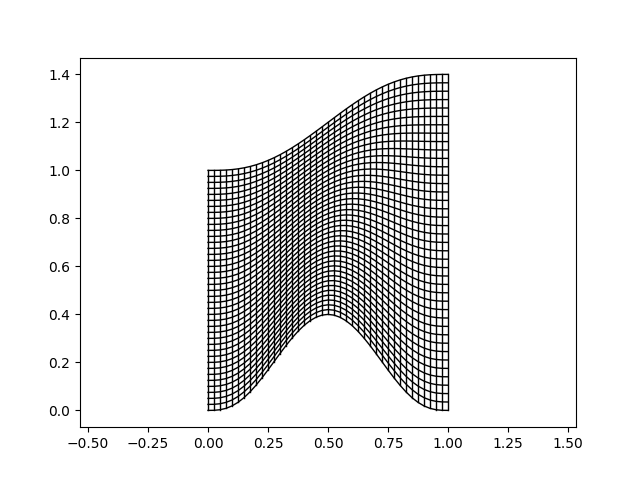
\includegraphics[width=.8\linewidth]{./2a.png}
\newpage 

\problemitem[2b)] Same with Hermite
\prob

Laziness ensues

\begin{verbatim}
"""
    The hermite interpolation between R0 (which now is a matrix containing the tangent 
    vectors as well
"""
function hermite(R0, R1, i)
    j= 3 - i
    R(xy) = [((2.0*xy[i]^3 - 3.0*xy[i]^2 + 1.0)*R0(xy[j])[:,1]
             +(xy[i]^3 - 2.0*xy[i]^2 + xy[i])*R0(xy[j])[:,2]
             +(-2.0*xy[i]^3 + 3.0*xy[i]^2)*R1(xy[j])[:,1]
             +(xy[i]^3 - xy[i]^2)*R1(xy[j])[:,2]) ((6.0*xy[i]^2 - 6.0*xy[i])*R0(xy[j])[:,1]
             +(3.0*xy[i]^2 - 4.0*xy[i] + 1.0)*R0(xy[j])[:,2]
             +(-6.0*xy[i]^2 + 6.0*xy[i])*R1(xy[j])[:,1]
             +(3.0*xy[i]^2 - 2.0*xy[i])*R1(xy[j])[:,2])]
    return R
end

"""
    This is the version of the above function that will work for the hermite guy
"""
function tfi_h(Fd, Fu, Fl, Fr, func)
    return xy -> func(Fd, Fu, 2)(xy)
end

"""
    Simply applying the tfi_h function above to the given example 
"""
function tfi_orthogonal(xy, A=0.4, T=0.5)
    return tfi_h(x->[[x,64.0*A*x^3*(1.0-x)^3] T*unit([6.0*64.0*A*(x-0.5)*x^2*(x-1.0)^2, 1.0])], 
               x->[[x,1+A*x^3*(6.0*x^2 - 15.0*x +10.0)] T*unit([-30.0*A*x^2*(x-1.0)^2, 1.0])], 
               y->[[0.0,y] T*[1.0, 0.0]], y->[[1.0,(1.0 + A)*y] T*[1.0, 0.0]], hermite)(xy)[:,1]
end
\end{verbatim}
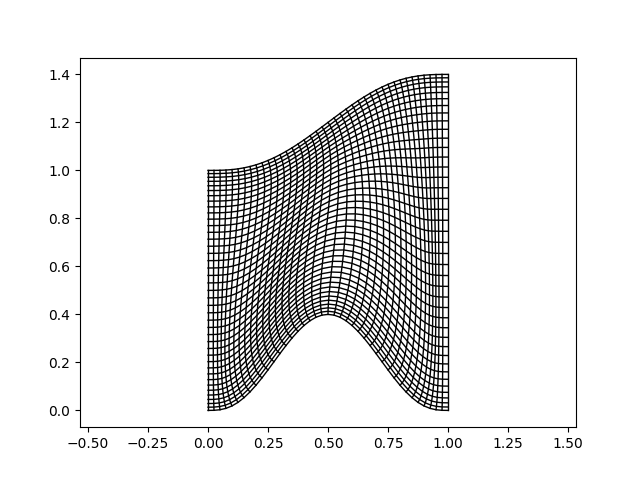
\includegraphics[width=.8\linewidth]{./2b.png}
\newpage% }}}
\problemitem[3)] Find the image of the rectangle $0 \leq \Re z \leq 1$, % {{{
$0 \leq \Im z \leq 2\pi$ under the mapping 
$$w = \frac{2e^z - 3}{3e^z - 2}.$$
Generate a structured grid of size $20 \times 80$ for this region with grid lines that 
are orthogonal everywhere.
\prob

We will consider this as the composition of the maps 
$$z \mapsto e^z \quad \text{and} \quad z \mapsto \frac{2z - 3}{3z - 2}$$
The first maps our square to an anulus of inner radius $1$ and outer radius $e$. This 
is because the real part of $z$ in $e^z$ controls the distance from 0, and the imaginary 
part controls the angle.

Now the second map is a M\"obius transformation which will send circles and lines 
to circles and lines which sends $3/2$ to $0$ and $2/3$ to $\infty$.

Since the coefficients are all real, the real line is sent to the real line and $\bar z$ is 
sent to the conjugate of where $z$ is sent. In particular, this means that circles with centers 
on the real axis will get sent to either circles with real center or vertical lines 
(if the center is the point that is sent to infinity). 

Thus we can easily calculate where the circles of radius $1$ and $e$ centered at zero are 
sent by looking at where $\pm 1$ and $\pm e$ are sent. (Note that our anulus is inverted 
because a point in the center is sent to infinity)
$$1 \mapsto \frac{2 - 3}{3 - 2} = -1, \qquad -1 \mapsto \frac{-2 - 3}{-3 - 2} = 1.$$
So actually, the radius 1 circle is mapped to itself! As for the other boundary:
$$e \mapsto \frac{2e - 3}{3e - 2} \approx 0.396, \qquad -e \mapsto \frac{-2e - 3}{-3e - 2} 
\approx 0.831.$$
Thus, our region is the unit disc with a disc centered at about 0.613 and radius about 0.217 
cut out of it! (It makes sense that 0 is in our region since $3/2$ started in our anulus!)

Finally, for the sake of graphing this mesh lets express the function as a real vector function
$$e^{x+iy} = e^x[\cos(y) + i\sin(y)]$$
$$2\Re \frac{2z - 3}{3z - 2} = \frac{2z - 3}{3z - 2} +\frac{2\bar z - 3}{3\bar z - 2}
= \frac{12 z \bar z - 13(z + \bar z) + 12}{9 z\bar z - 6(z + \bar z) + 4}
= 2\frac{6 \abs{z}^2 - 13 \Re z + 6}{9 \abs{z}^2 - 12 \Re z + 4}$$
$$2\Im \frac{2z - 3}{3z - 2} = \frac{2z - 3}{3z - 2} -\frac{2\bar z - 3}{3\bar z - 2}
= \frac{5(z + \bar z)}{9 z\bar z - 6(z + \bar z) + 4}
= 2\frac{5 \Im z}{9 \abs{z}^2 - 12 \Re z + 4}$$

Here is a plot using the provided utility:

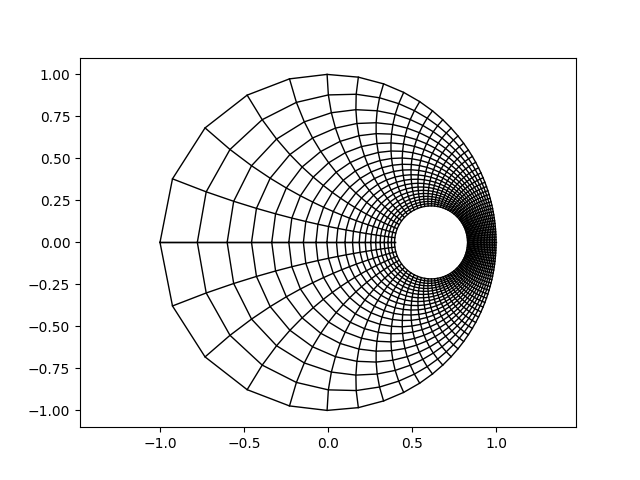
\includegraphics[width=.8\linewidth]{./meromorph.png}
\newpage
% }}}
\problemitem[4)] Write the mesher
\prob

\begin{flushright}
\begin{verbatim}
"""
    Takes a matrix (although I feel like a vector of vectors is more natural but whatever)
    pv whose rows are coordinates of boundary points in order around the boundary 
    and triangulates with roughly Delaunay triangles of max area less than hmax^2/2^(nref+1) 
    and side length approximately hmax/2^(nref)
"""
function pmesh(pv, hmax::Float64, nref)
    ps = Vector{Float64}[] # this will be a vector of points 
    for i in (1:size(pv)[1]-1)
        dist = (x->sqrt(x'*x))(pv[i,:] - pv[i+1,:]) # the distance between point i and i+1
        n = ceil(dist / hmax)
        append!(ps, [pv[i,:]*(1.0 - k/n) + pv[i+1,:]*k/n for k in (0:n-1)]) #linear interpolation
    end
    while true
        t = map(x -> collect(x), D.triangulate(ps).triangles) # collect the tuples into vectors
        t = filter(x -> inpolygon(masscenter(ps[x]), pv) && area(ps[x]) >= 10^(-12), t)
                   
        largest = findfirst(x -> area(ps[x]) > hmax^2/2, t)
        if isnothing(largest)
            for i in (1:nref)
                edges, _, _ = all_edges(hcat(t...)')
                for e in [edges[i, :] for i in (1:size(edges)[1])]
                    push!(ps, masscenter(ps[e]))
                end
                t = map(x -> collect(x), D.triangulate(ps).triangles)
                t = filter(x -> inpolygon(masscenter(ps[x]), pv) && area(ps[x]) >= 10^(-12), t)
            end
            return hcat(ps...)', hcat(t...)', boundary_nodes(hcat(t...)')
        end
        push!(ps, circumcenter(ps[t[largest]]))
    end
end

"""
    The circumcenter of a triangle to be sure Delaunay deletes the bad triangle. The circumcenter 
    is the unique point that makes lies on the perpendicular bisector of all lines, which is 
    a quick matrix inversion

    I'm not sure we're supposed to be using the circumcenter right? What 
    if Delaunay makes a big triangle on the border, then the circumcenter 
    is (maybe) outside the convex hull of the shape?!
"""
function circumcenter(ps)
    m12 = (ps[1] + ps[2])/2.0
    m13 = (ps[1] + ps[3])/2.0
    d12 = (ps[1] - ps[2])
    d13 = (ps[1] - ps[3])
    return hcat(d12, d13)' \ [d12' * m12, d13' * m13]
end

"""
    To check outside triangles we use the center of mass which is always in the interior of a 
    triangle, although I'm realizing now that this might not work in general. I guess it's fine 
    because Delaunay will always make a planar graph so any triangle is either completely 
    inside or outside the desired shape (but only if Delaunay keeps the edges?) Whatever, 
    time to turn in
"""
function masscenter(ps)
    return sum(ps)/length(ps)
end

"""
    Use the wedge product to compute the area of a triangle
"""
function area(ps)
    d12 = (ps[1] - ps[2])
    d13 = (ps[1] - ps[3])
    return 0.5 * abs(d12[1]*d13[2] - d12[2]*d13[1])
end


\end{verbatim}
\end{flushright}
\end{problems}
\end{document}
